\documentclass[oneside]{book}
\usepackage{amsmath,amssymb}
\usepackage{algorithm,algorithmic}
\usepackage{graphicx}
\usepackage{listings}
\usepackage{color}
\usepackage{fullpage}

\definecolor{dkgreen}{rgb}{0,0.6,0}
\definecolor{gray}{rgb}{0.5,0.5,0.5}
\definecolor{mauve}{rgb}{0.58,0,0.82}

\lstset{frame=tb,
  language=Java,
  aboveskip=3mm,
  belowskip=3mm,
  showstringspaces=false,
  columns=flexible,
  basicstyle={\small\ttfamily},
  numbers=none,
  numberstyle=\tiny\color{gray},
  keywordstyle=\color{blue},
  commentstyle=\color{dkgreen},
  stringstyle=\color{mauve},
  breaklines=true,
  breakatwhitespace=true
  tabsize=0
}
\begin{document}

\title{\textbf{CS3410: Software Engineering Lab}\\ \textbf{LR(1) parser for JavaCC}}
\author{Aravind S CS11B033\\
    Akshayaram S CS11B057 \\
    Srinivasan R CS11B059 \\
    Ramnandan SK CS11B061 \\
    Adit Krishnan CS11B063
}

\maketitle

\tableofcontents

\chapter{Introduction}
\section{Context Free Grammars}
A Context Free Grammars (CFG) consists of Terminals, Non-terminals, Start Symbol and Productions.
\begin{enumerate}
\item Terminals are the basic symbols from which strings of the language are formed. Terminals are also called as tokens and correspond to the tokens that are returned by the lexical analyzer.
\item Non-Terminals are syntactic variables that denote a set of strings. Non-terminals impose a hierarchical structure on the language that is key to syntax analysis and translation.
\item A non-terminal is distinguished as the start symbol and the set of strings that are derived from the start symbol comprises of the language.
\item The productions of a grammar specify the manner in which terminals and non-terminals are combined to form strings. In a CFG:
\begin{itemize}
\item A single non-terminal to the left side of the production which is called as the head or the lhs.
\item The body or the rhs which comprises of zero or more non-terminals and terminals.
\end{itemize} 
\end{enumerate}

\subsection{Derivations}
A derivation is composed of the set of productions that must be applied to get a given string belonging to the language starting at the start symbol.

A \textit{leftmost derivation} is one in which the leftmost non-terminal is replaced with the right hand side of the production involving the non-terminal.

A \textit{rightmost derivation} is one in which the rightmost non-terminal is replaced with the right hand side of the production involving the non-terminal.

\section{Lexical Analyzers and Parsers}
 Parsers and lexical analyzers are the first two components that are present in the front end of any compiler. \textit{Lexical analyzer} reads a stream of characters from the source program and groups the characters into meaningful sequences called as \textit{tokens} which is passed to the next phase of the compiler which is the parser.  

\textit{Parser} or the syntax analyzer uses the tokens produced by the lexical analyzer to produce a tree-like intermediate representation which depicts the grammatical structure of the token stream. A typical representation is that of a syntax tree in which each interior node represents an operation and the leaves represent the operands or the arguments.

\subsection{Top Down Parsing}
 Top down parsing can be viewed as the problem of generating the parse tree for the input string in the depth first order starting at the root. The class of grammars for which one could construct predictive top down parsers with $k$ look ahead symbols is called as $LL(k)$ grammars where first $L$ refers to the left to right scanning, the second $L$ stands for leftmost derivation and $k$ refers to the number of lookahead tokens used in decision making.
 
 \subsubsection*{$LL(k)$ Grammars}
 A Context Free Grammar is called $LL(k)$ if and only if for all non-terminals $A$ and each distinct pair of production $A \rightarrow \beta$ and $A \rightarrow \gamma$ satisfy the condition $First_k(\beta) \cap First_k(\gamma) = \phi$ where $First_k(\alpha)$ the set of $k$ terminals that occur in the beginning in all strings derived from non-terminal $\alpha$.
 
 It is a well known fact that predictive parsers i.e recursive decent parsers can be constructed for $LL(k)$ grammars without backtracking and requiring $k$ lookahead tokens. $LL(k)$ parsers are easy to generate and are very efficient parsers can be generated for $LL(k)$ grammars. But it suffers from the following drawbacks:
 
 \begin{enumerate}
 \item It cannot parse any left recursive grammar.
 \item It cannot parse any ambiguous grammar (An ambiguous grammar is one in which there exists a string in the language generated by the grammar which has at least two different parse trees)
 \item Some languages have no $LL(k)$ grammars.
 
 \end{enumerate}
 
 \subsection{Bottom Up Parsing}
 A bottom up parsing corresponds to constructing a parse tree for an input from the leaves and working towards the root. One can think of bottom up parsing as a process of reducing a string to the start symbol of the grammar. The most common grammars that can be parsed with a bottom up parser is called as the $LR(k)$ parsers where first $L$ refers to left to right scanning of input, $R$ refers to constructing reverse rightmost derivation and $k$ is the number of lookahead symbols.
 
\subsubsection*{$LR(k)$ Grammars} 

A grammar is said to be $LR(k)$ if given a rightmost derivation 
$$
S = \gamma_0 \Rightarrow \gamma_1 \Rightarrow \gamma_2 \Rightarrow \cdots \gamma_k = w
$$
we can determine for each right sentential form in the derivation
\begin{itemize}
\item The handle to used 
\item The production to be used for reduction  
\end{itemize}
by scanning $\gamma_i$ from left to right and scanning at most $k$ symbols beyond right end of the handle $\gamma_i$.

We will look into more details of $LR(k)$ grammar in the next chapter.

\section{JavaCC}
JavaCC is a parser generator and a lexical analyzer written in Java programming language. It is a open source project and is similar to yacc in that it generates a parser from the formal grammar written in Extended Backus-Naur form (EBNF). JavaCC generates top down parsers and hence limited to parsing only $LL(k)$ grammars and hence cannot parse left recursive grammars. Some of the highlights of JavaCC are:

\begin{enumerate}
\item JavaCC enjoys a large user community and is by far the most widely used parser generator for Java applications.
\item An important feature of JavaCC is that both the lexical specification such as token, regular expressions, strings and the BNF for the grammar can be specified in the same file unlike the flex-Bison combination where the lexical specifications and the grammar specification are written in separate files.
\item JavaCC comes with JJtree which is an extremely powerful tree processor. It converts the given grammar file to a parse tree with internal nodes indicating the non-terminals and the leaves indicating the terminals.
\item By default JavaCC generates an $LL(1)$ parser but it is highly customizable and one can specify the number of lookahead tokens ($k$) to be used just before running it on a specific grammar file.  
\end{enumerate}
 
 JavaCC uses $LL(k)$ parser and hence cannot parse a lot of languages that can be parsed only by a $LR(1)$ parser (for example left recursive grammars). Hence, we wanted to write a $LR(1)$ parser for a restrictive choice of grammars for JavaCC.
 
 \chapter{LR(1) parsers}

This chapter gives a brief introduction about $LR(1)$ parsing algorithms and constructing the $LR(1)$ parser table that we used in writing a $LR(1)$ parser for JavaCC. Before we go into the construction, we wish to specify a few definitions and notations that we will be using throughout the chapter. We have referred extensively to \cite{aho1985} for the algorithms and the techniques explained in this chapter.

\section{Preliminaries}
Bottom up parsing or $LR(1)$ parsing is the process of \textit{reducing} a string $w$ to start symbol by applying a series of production rules. At each \textit{reduction} step, a specific substring matching the rhs of a production is replaced with the a non-terminal corresponding to the lhs or the head of the production.

Bottom up parsing during a left to right scan of the input constructs a rightmost derivation in reverse. A \textit{handle} is a substring that matches the body of a production and whose reduction represents one step in the reverse rightmost derivation.

$First(\alpha)$ is defined as the set of terminals that begin strings derived from $\alpha$. If $\alpha \Rightarrow \epsilon$, then $\epsilon \in First(\alpha)$.

\section{Shift-Reduce Parsing}
Shift-reduce parsing is a form of bottom up parsing in which a stack holds a set of grammar symbols and buffer contains the rest of the input that is to be parsed. 

Informally, during a left to right scan of the input the parser shifts 0 or more symbols to the top of the stack until it is ready to reduce a string $\beta$ of grammar symbols on top of the stack. It then reduces $\beta$ to the head of appropriate production. The parser repeats this until it has detected an error or the stack consists of the start symbol and the buffer is empty.

A shift-reduce parser has four canonical actions:

\begin{itemize}
\item \textit{Shift}: Shift the next input on top of the stack.
\item \textit{Reduce}: Right end of the handle is on top of the stack. Locate the left end of the handle within the stack. Pop the handle off the stack and push the appropriate non-terminal into the stack.
\item \textit{Accept:} Accepts the successful parsing of the given string.
\item \textit{Reject:} Discover a syntax error and call the error recovery routine.
\end{itemize}

\begin{algorithm}
\caption{Shift-Reduce Parser}
\begin{algorithmic}
\REQUIRE Goto table, action table and string w. 
\STATE push $s_0$
\STATE $token \leftarrow next\_token()$ 
\WHILE{true}
\STATE $s \leftarrow $ top of stack
\IF{$action[s,token] = $ "shift $s_i$"}
\STATE push $s_i$
\STATE $token \leftarrow next\_token()$ 
\ELSIF{$action[s,token] = $ "reduce $A \rightarrow \beta$"}
\STATE pop $|\beta|$ states from the stack
\STATE $s' = $ top of the stack
\STATE push $goto[s',A]$
\ELSIF{$action[s,token] = $ "accept"}
\STATE return
\ELSE
\STATE error()
\ENDIF
\ENDWHILE
\end{algorithmic}
\end{algorithm}

\section{Computing First of a non-terminal}
We now give an algorithm for computing the first set of a non-terminal.

\begin{algorithm}
\caption{Computing $First(X)$}
\begin{algorithmic}
\IF{$X$ is terminal}
\STATE $FIRST(X) = X$
\ENDIF
\IF{$X \Rightarrow \epsilon$}
\STATE Add $\epsilon$ to $First(X)$.
\ENDIF
\IF{$X \Rightarrow Y_1Y_2...Y_k$}
\STATE Add $First(Y_1) - \epsilon$ to $FIRST(X)$
\FOR{i = 1 to k}
\IF{$Y_1Y_2...Y_{i} \Rightarrow \epsilon$}
\STATE Add $First(Y_{i+1}) - \epsilon$ to $FIRST(X)$
\ENDIF
\ENDFOR
\IF{$Y_1Y_2...Y_{k} \Rightarrow \epsilon$}
\STATE Add $\epsilon$ to $FIRST(X)$
\ENDIF
\ENDIF
\end{algorithmic}
\end{algorithm}

\section{$LR(1)$ items}

A $LR(1)$ item is pair $[\alpha,\beta]$ where 
\begin{itemize}
\item $\alpha$ is a production in $G$ with a $\bullet$ at some position in the rhs indicating how much of the input has been read.
\item $\beta$ is the lookahead symbol.
\end{itemize}

\subsection{$Closure1(I)$}
Given an item $[A \rightarrow \alpha \bullet B \beta, a]$ its closure contains the item and any other items that can generate legal substrings to follow $\alpha$. We now provide the algorithm for computing the closure.

\begin{algorithm}
\caption{Computing $Closure1(I)$}
\begin{algorithmic}
\REPEAT
\IF{$[A \rightarrow \alpha \bullet B \beta, a] \in I$}
\STATE Add $[B \rightarrow \bullet \gamma, b]$ to $I$ where $b \in First(\beta a)$
\ENDIF
\UNTIL{no more items can be added to $I$}
\end{algorithmic}
\end{algorithm}

\subsection{$Goto1(I)$}
Let $I$ be a set of $LR(1)$ items and $X$ be a grammar symbol. $Goto1(I,X)$ is the closure of $[A \rightarrow \alpha X \bullet \beta]$ such that $[A \rightarrow \alpha\bullet X  \beta] \in I$

We now give the algorithm for computing the $Goto1(I,X)$

\begin{algorithm}
\caption{$Goto1(I,X)$}
\begin{algorithmic}
\STATE Let $J$ be the set of items $[A \rightarrow \alpha X \bullet \beta]$ such that $[A \rightarrow \alpha\bullet X  \beta] \in I$.
\STATE return $Closure1(J)$
\end{algorithmic}
\end{algorithm}

\subsection{Computing $LR(1)$ item sets}
Now, we give the algorithm for computing the $LR(1)$ item sets.

\begin{algorithm}
\caption{Computing $LR(1)$ item sets}
\begin{algorithmic}
\STATE $s_0 \leftarrow Closure1([S' \rightarrow \bullet S, \$]$
\STATE $C \rightarrow \{s_0\}$
\REPEAT
\FOR{each set of items $s \in C$}
\FOR{each grammar symbol $X$}
\IF{$Goto1(s,X) \neq \phi$ and $Goto1(s,X) \notin C$}
\STATE Add $Goto1(s,X)$ to $C$
\ENDIF 
\ENDFOR
\ENDFOR 
\UNTIL{no more sets can be added to $C$}
\STATE return $C$ 
\end{algorithmic}
\end{algorithm}  

\subsection{$LR(1)$ parser}
We now give the algorithm for constructing the $LR(1)$ parsing table.
\begin{algorithm}
\caption{$LR(1)$ parsing table}
\begin{algorithmic}
\STATE $C \leftarrow$ Compute $LR(1)$ item sets
\IF{$[A \rightarrow \alpha \bullet a,  \beta] \in I_i$ and $Goto1(I_i,a) = I_j$}
\STATE $action[I_i,a] \leftarrow$ "shift $I_j$"
\ENDIF
\IF{$[A \rightarrow \alpha \bullet,  a] \in I_i$ and $A \neq S'$}
\STATE $action[I_i,a] \leftarrow$ "reduce $A \rightarrow \alpha$"
\ENDIF
\IF{$[S \rightarrow S' \bullet,  \$] \in I_i$ }
\STATE $action[I_i,a] \leftarrow$ "accept"
\ENDIF
\IF{$Goto1[I_i,a] = I_j$}  
\STATE $Goto[I_i,a] = I_j$
\ENDIF
\STATE set undefined entries to error.
\STATE Initial state is $s_0 \leftarrow Closure1([S' \rightarrow \bullet S, \$)$
\end{algorithmic}
\end{algorithm}  

\chapter{Class hierarchies and Design Patterns}
\section{Outline of the code}
The code for the parser in JavaCC was written in src/org/javacc/parser.The various options that govern the parser like lookahead, debug-enable, etc are taken as input and pushed into a class \texttt{Options}.\\\\We skip over the tokenization portion as it is not relevant to us. We only need to know the API updated by the tokenizer. Before the parser is called, the tokens and productions are updated in global constructs in \texttt{JavaCCGlobals}. The suitable containers for Tokens and Productions can be found in the \texttt{Token} and \texttt{NormalProduction} respectively. Productions supplied in the \texttt{.jj} file to be parsed may be Java code as well in which we have a sub-class for Productions called \texttt{JavaCodeProduction}. A similar case holds for \texttt{BNFProduction} as well.\\\\The RHS's of productions is generically called \texttt{Expansion} which can again be of several types and hence has sub-classes:
\begin{enumerate}
\item \texttt{Choice} for \texttt{|} in a RegEx
\item \texttt{Non-Terminal}
\item \texttt{OneOrMore} for \texttt{+} in a RegEx
\item \texttt{RegularExpression}
\item \texttt{Sequence} for a sequence of any of these
\item \texttt{ZeroOrMore} for \texttt{*} in a RegEx
\item \texttt{ZeroOrOne} for \texttt{?} in a RegEx
\item \texttt{TryBlock} for a try-catch block
\end{enumerate}
\noindent For example: \texttt{(<id>+|$\backslash$n)($\backslash$t)*} would throw up firstly a \texttt{Sequence}, the first of which is a \texttt{Choice} of a \texttt{OneOrMore} and a simple token, and the second of which is a \texttt{ZeroOrMore}.\\\\\texttt{RegularExpression} also has similar sub-classes for the same reason and these files are prefixed with an \texttt{R} in their name.\\\\Another notable point is that the code allows for C++-specific constructs as well and this is specifically handled everywhere in the code.\\\\Now, let's walk through a typical run. As always, the \texttt{Main} class begins the process. After some initializations, \texttt{ParseGen} is called (note that there are variants for CPP like \texttt{ParseGenCPP}) after which a Lexer is also generated (using \texttt{LexGen} or \texttt{LexGenCPP}) but we will not delve into the lexing.\\\\\texttt{ParseGen} mainly does some tertiary code dumping amidst which it invokes \texttt{ParseEngine} which is the heart of the parser generator. This file contains functions which build First sets and generate code to do LL(k) parsing. The function \texttt{buildLookaheadChecker()} does this work which has a mini-state machine to generate the suitable lookahead sequences.\\\\Another notable feature is the use of buffers which hold portions of the code which are dumped at requisite points of time. Also, file \texttt{JavaCC.jj} contains the grammar and actions that describe \texttt{JavaCCParser}. When passed as input to \texttt{JavaCCParser} it generates another copy of itself.
%When we analyzed the code written for the parser in JavaCC we found that predominantly Abstract factory and Factory method used most often.

\section{Class Hierarchies}
In this section we present the class hierarchies and in the next present the interactions amongst these and observe the various design patterns.
\begin{center}
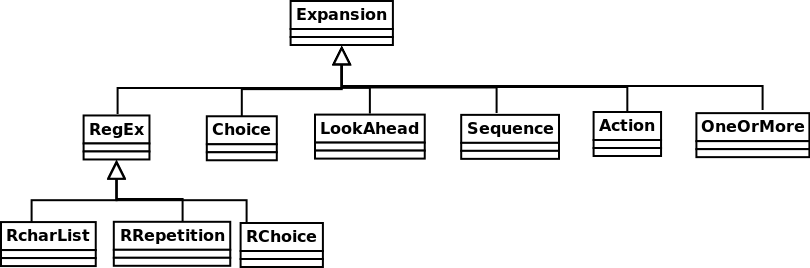
\includegraphics[scale=0.5]{Expansion.png}
\end{center}

\begin{center}
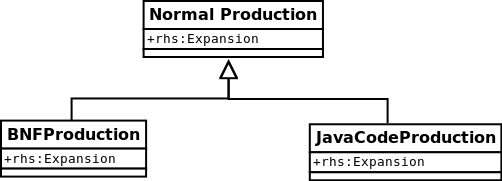
\includegraphics[scale=0.5]{NormalProduction.png}
\end{center}

\begin{center}
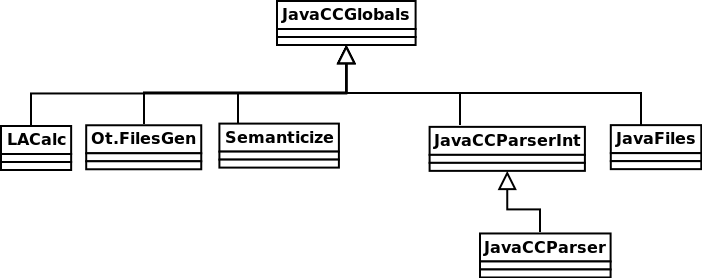
\includegraphics[scale=0.5]{javaCCGlobals.png}
\end{center}

\begin{center}
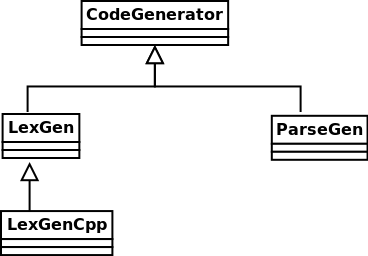
\includegraphics[scale=0.5]{CodeGenerator.png}
\end{center}

\section{Design Patterns}
In software engineering, is a generic reusable solution to a commonly occurring problem within a software engineering domain. Design patterns were formally introduced in the book Design Patterns: Elements of reusable Object Oriented Software which was published in 1994 by Gamma et al.\cite{gamma1994}.

Design patterns are broadly classified into structural, creational and behavioral patterns.

As we went through the code in JavaCC parser folder we came across one instance of \textit{Builder Pattern} and one instance of \textit{Factory Method} which are explained below.

\subsection{Builder Pattern}
Builder pattern is used when there is a construction of a complex object from its representation so that the same construction process can be used to create different representations depending on the input.

It is used when,
\begin{itemize}
\item There is an algorithm for creating a complex object which is independent of the parts that make up the object.
\item The above algorithm must allow different representations of constructing the complex object.
\end{itemize}

\begin{center}
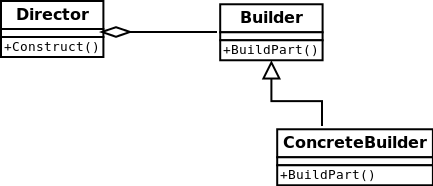
\includegraphics[scale=0.5]{Builder.png}
\end{center}

The participants are:
\begin{itemize}
\item \textbf{Builder} Specifies the abstract interface for creating an object
\item \textbf{Concrete Builder} Implements the builder interface and keeps track of the representation it creates
\item \textbf{Director} Creates objects using builder interface.
\end{itemize}

\subsection{Factory Method}
According to \cite{gamma1994}, a factory method is used to define an interface for creating an object, but let subclasses decide which class to instantiate. Factory Method lets a
class defer instantiation to subclasses.
 Factory methods are used when:
 \begin{enumerate}
 \item A class can't anticipate the class of objects that it must create
 \item A class wants its subclasses to specify the object or the product it creates.
 \item Classes delegate responsibility to one of several helper subclasses, and you want to localize the knowledge of
which helper subclass is the delegate.
 \end{enumerate}
 
 The class diagram for a Factory Method is as follows.
 \begin{center}
 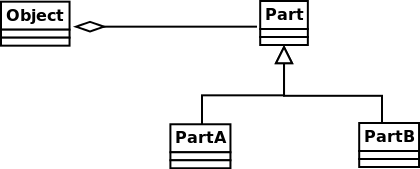
\includegraphics[scale=0.5]{FactoryMethod.png}
 \end{center}
 
 The participants are:
 \begin{itemize}
 \item \textbf{Object}: It defines the interface of the product that the factory method creates
 \item \textbf{Part:} It defines the interface of the part that the factory method creates.

 \end{itemize}

\subsection{Design Patterns Observed}

We could observe the following design patterns between classes defined in parser folder.

\subsubsection*{Builder} 

Based on the token that it receives at the run-time Normal Production either builds up a choice or regEx or Sequence and so on. Hence, this is an example of the builder pattern.
\begin{center}
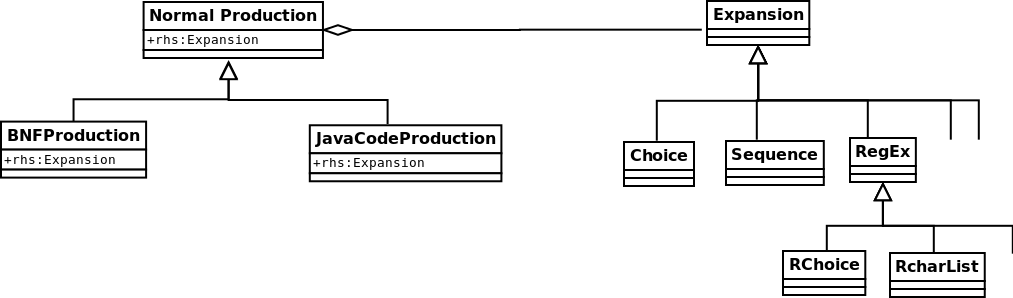
\includegraphics[scale=0.4]{AbstractFactory1.png}
\end{center} 

\subsubsection*{Factory Method}
\begin{center}
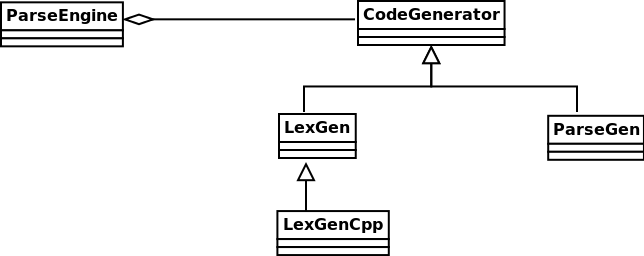
\includegraphics[scale=0.5]{FactoryMethod1.png}
\end{center}

\chapter{Code Added}
We had implemented $LR(1)$ parser for a restricted set of CFG grammars. The CFG grammars that can be currently parsed by the $LR(1)$ parser that we have built are those which do not have a choice in any of the productions.

The file which was earlier implementing the $LL(k)$ parser was the ParseEngine.java and that is where we had made most of the changes. We had defined two new classes called as the Item and ItemSet to construct the $LR(1)$ items.\\


We then added functions in the ParseEngine.java file to compute the Closure1, Goto1, build the $LR(1)$ table, constructing the $Goto1$ table and finally for code emission. In essence, we had implemented all the algorithms that have been highlighted in chapter-2. We give the details of all the code added in the appendix.

\chapter*{Appendix}
\textbf{Item.java}
\begin{lstlisting}

package org.javacc.parser;

public class Item {
  private NormalProduction p = new NormalProduction();
  private int offset = 0;
  private int la;
  private boolean isFirst = false;
  private boolean isLast = false;

  
  public boolean isFirst() {
    return isFirst;
  }
  public void setFirst(boolean isFirst) {
    this.isFirst = isFirst;
  }
  public boolean isLast() {
    return isLast;
  }
  public void setLast(boolean isLast) {
    this.isLast = isLast;
  }
  public int getOffset() {
    return offset;
  }
  public void setOffset(int offset) {
    this.offset = offset;
  }
  public NormalProduction getP() {
    return p;
  }
  public void setP(NormalProduction p) {
    this.p = p;
  }
  public int getLa() {
    return la;
  }
  public void setLa(int la) {
    this.la = la;
  }
  

}

\end{lstlisting}

\textbf{ItemSet.java}

\begin{lstlisting}
package org.javacc.parser;

import java.util.*;

public class ItemSet {
  private int index;
  private List<Item> itemSet = new ArrayList<Item>();
  public List<Item> getItemSet() {
    return itemSet;
  }
  public void setItemSet(List<Item> itemSet) {
    this.itemSet = itemSet;
  }
  public int getIndex() {
    return index;
  }
  public void setIndex(int index) {
    this.index = index;
  }
}

\end{lstlisting}

\textbf{Computing the closure of the $Item_0$}

\begin{lstlisting}
public ItemSet buildClosure() {
    boolean flag = false;
    String lhsNT = "";
    Set<String> seen = new HashSet<String>();
    Set<NormalProduction> seen_production = new HashSet<NormalProduction>();
    
    Item first = new Item();
    first.setFirst(true);
    
    Item last = new Item();
    last.setLast(true);
    
    ItemSet itemSet = new ItemSet();
    itemSet.getItemSet().add(first);
    
    Item firstItem = new Item();
    firstItem.setP((NormalProduction)bnfproductions.get(0));
    firstItem.setOffset(0);
    firstItem.setLa(0);
    itemSet.getItemSet().add(firstItem);
    
    // TODO: Check for choices on S ->
    
    do {
      flag = false;
      ItemSet temp = new ItemSet();
      for(Item i : itemSet.getItemSet()) {
        if(!i.isFirst() && !i.isLast()) {
          lhsNT = "";
          if(i.getOffset() < ((Sequence) i.getP().getExpansion()).units.size() - 1 && ((Sequence) i.getP().getExpansion()).units.get(i.getOffset() + 1) instanceof NonTerminal) {
            // matching the LHS and getting the productions whose hed is same as lhsNT
            lhsNT += ((NonTerminal)((Sequence) i.getP().getExpansion()).units.get(i.getOffset() + 1)).getName();
            if(((Sequence) i.getP().getExpansion()).units.size() == i.getOffset() + 2) {
              for(int k = 0; k < bnfproductions.size(); k++) {
                NormalProduction normalProduction = (NormalProduction)bnfproductions.get(k);
                if(normalProduction.getLhs().equals(lhsNT)) {
                  Item item = new Item();
                  item.setP(normalProduction);
                  item.setOffset(0);
                  item.setLa(i.getLa());
                  temp.getItemSet().add(item);
                }                
              }
            } else if(((Sequence) i.getP().getExpansion()).units.get(i.getOffset() + 2) instanceof NonTerminal) {
              if(!seen.contains(lhsNT)) {
                seen.add(lhsNT);
                flag = true;
              
                if (firstSet == null) {
                  firstSet = new boolean[tokenCount];
                }
              
                for (int j = 0; j < tokenCount; j++) {
                  firstSet[j] = false;
                }
          
                genFirstSet((NonTerminal)((Sequence) i.getP().getExpansion()).units.get(i.getOffset() + 2));
              
                for(int k = 0; k < bnfproductions.size(); k++) {
                  NormalProduction normalProduction = (NormalProduction)bnfproductions.get(k);
                  for (int j = 0; j < tokenCount; j++) {
                    if(normalProduction.getLhs().equals(lhsNT) && firstSet[j] == true) {
                      Item item = new Item();
                      item.setP(normalProduction);
                      item.setOffset(0);
                      item.setLa(j);
                      temp.getItemSet().add(item);
                    }
                  }
                }
              }
            } else {
              for(int k = 0; k < bnfproductions.size(); k++) {
                NormalProduction normalProduction = (NormalProduction)bnfproductions.get(k);
                if(normalProduction.getLhs().equals(lhsNT)) {
                  if(!seen_production.contains(normalProduction)) {                
                    Item item = new Item();
                    item.setP(normalProduction);
                    item.setOffset(0);
                    item.setLa(((RegularExpression)((Sequence) i.getP().getExpansion()).units.get(i.getOffset() + 2)).ordinal);
                    temp.getItemSet().add(item);
                    flag = true;
                    seen_production.add(normalProduction);
                  }
                }
              }
            }
          }
        }
      }
      
      itemSet.getItemSet().addAll(temp.getItemSet());
    } while(flag);
    
    return itemSet;
  }
\end{lstlisting}

\textbf{Computing Closure of other ItemSets}
\begin{lstlisting}
public void buildClosureOthers(ItemSet its) {
    boolean flag = false;
    String lhsNT = "";
    Set<String> seen = new HashSet<String>();
    Set<NormalProduction> seen_p = new HashSet<NormalProduction>();
    
    do {
      flag = false;
      ItemSet temp = new ItemSet();
      for(Item i : its.getItemSet()) {
        if(!i.isFirst() && !i.isLast()) {
          lhsNT = "";
          if(i.getOffset() < ((Sequence) i.getP().getExpansion()).units.size() - 1 && ((Sequence) i.getP().getExpansion()).units.get(i.getOffset() + 1) instanceof NonTerminal) {
            lhsNT += ((NonTerminal)((Sequence) i.getP().getExpansion()).units.get(i.getOffset() + 1)).getName();
            if(((Sequence) i.getP().getExpansion()).units.size() == i.getOffset() + 2) {
              for(int k = 0; k < bnfproductions.size(); k++) {
                NormalProduction np = (NormalProduction)bnfproductions.get(k);
                if(np.getLhs().equals(lhsNT)) {
                  Item item = new Item();
                  item.setP(np);
                  item.setOffset(0);
                  item.setLa(i.getLa());
                  temp.getItemSet().add(item);
                }                
              }
            } else if(((Sequence) i.getP().getExpansion()).units.get(i.getOffset() + 2) instanceof NonTerminal) {
              if(!seen.contains(lhsNT)) {
                seen.add(lhsNT);
                flag = true;
              
                if (firstSet == null) {
                  firstSet = new boolean[tokenCount];
                }
              
                for (int j = 0; j < tokenCount; j++) {
                  firstSet[j] = false;
                }
          
                genFirstSet((NonTerminal)((Sequence) i.getP().getExpansion()).units.get(i.getOffset() + 2));
              
                for(int k = 0; k < bnfproductions.size(); k++) {
                  NormalProduction np = (NormalProduction)bnfproductions.get(k);
                  for (int j = 0; j < tokenCount; j++) {
                    if(np.getLhs().equals(lhsNT) && firstSet[j] == true) {
                      Item item = new Item();
                      item.setP(np);
                      item.setOffset(0);
                      item.setLa(j);
                      temp.getItemSet().add(item);
                    }
                  }
                }
              }
            } else {
              for(int k = 0; k < bnfproductions.size(); k++) {
                NormalProduction np = (NormalProduction)bnfproductions.get(k);
                if(np.getLhs().equals(lhsNT)) {
                  if(!seen_p.contains(np)) {                
                    Item item = new Item();
                    item.setP(np);
                    item.setOffset(0);
                    item.setLa(((RegularExpression)((Sequence) i.getP().getExpansion()).units.get(i.getOffset() + 2)).ordinal);
                    temp.getItemSet().add(item);
                    flag = true;
                    seen_p.add(np);
                  }
                }
              }
            }
          }
        }
      }
      
      its.getItemSet().addAll(temp.getItemSet());
    } while(flag);  
  }
\end{lstlisting}

\textbf{Computing Goto for a Non-terminal}
\begin{lstlisting}
public ItemSet computeGotoNonTerminal(ItemSet I, String s, boolean using_result) {
    ItemSet returnedItemSet = new ItemSet();
    
    for(Item item : I.getItemSet()) {
      if(!item.isFirst() && !item.isLast()) {
        for(int j = 0; j < ((Sequence) item.getP().getExpansion()).units.size(); j++) {
          if(((Sequence) item.getP().getExpansion()).units.get(j) instanceof NonTerminal) {
            if(s.equals(((NonTerminal)((Sequence) item.getP().getExpansion()).units.get(j)).getName()) && item.getOffset() == j - 1) {
              
              Item newItem = new Item();
              newItem.setP(item.getP());
              newItem.setOffset(item.getOffset() + 1);
              newItem.setLa(item.getLa());
              returnedItemSet.getItemSet().add(newItem);
            }
          }
        }
      }
      
      if(added_last_item == false && item.isFirst() && s.equals(((NormalProduction)bnfproductions.get(0)).getLhs())) {
        Item newItem = new Item();
        newItem.setLast(true);
        returnedItemSet.getItemSet().add(newItem);
        
        if(using_result == true) {
          added_last_item = true;
        }
      }
    }
    
    buildClosureOthers(returnedItemSet);
    
    return returnedItemSet;
  }
\end{lstlisting}
\textbf{Computing Goto for terminal}
\begin{lstlisting}
public ItemSet computeGotoRegEx(ItemSet I, int ind) {
    ItemSet ret = new ItemSet();
    
    for(Item i : I.getItemSet()) {
      if(!i.isFirst() && !i.isLast()) {
        for(int j = 0; j < ((Sequence) i.getP().getExpansion()).units.size(); j++) {
          if(((Sequence) i.getP().getExpansion()).units.get(j) instanceof RStringLiteral) {
            if(ind == ((RegularExpression)((Sequence) i.getP().getExpansion()).units.get(j)).ordinal && i.getOffset() == j - 1) {
            
              Item h = new Item();
              h.setP(i.getP());
              h.setOffset(i.getOffset() + 1);
              h.setLa(i.getLa());
              ret.getItemSet().add(h);
            }
          }
        }
      }
    }
    
    buildClosureOthers(ret);
    
    return ret;
  }
\end{lstlisting}

\textbf{Computing the Item Sets}
\begin{lstlisting}
public void computeItemSets() {
    ItemSet item_0 = buildClosure();
    boolean flag = false;
    int index = 1;
    
    item_0.setIndex(0);
    itemSets.add(item_0);
    
    List<ItemSet> temp = new ArrayList<ItemSet>();
    
    for(int i = 0; i < bnfproductions.size(); i++) {
      NormalProduction normalProduction = (NormalProduction)bnfproductions.get(i);
      if(!NT.contains(normalProduction.getLhs())) {
        NT.add(normalProduction.getLhs());
      }
    }
    
    do {
      flag = false;
      temp.clear();
      for(ItemSet itemSet : itemSets) {
        for(String X : NT) {
          if(computeGotoNonTerminal(itemSet, X, false).getItemSet().size() != 0 && !ourContains(itemSets, computeGotoNonTerminal(itemSet, X, false))) {
            ItemSet newItemSet = new ItemSet();
            newItemSet.getItemSet().addAll(computeGotoNonTerminal(itemSet, X, true).getItemSet());
            newItemSet.setIndex(index);
            index++;
            temp.add(newItemSet);
            flag = true;
          }
        }
        
        for(int X = 0; X < tokenCount; X++) {
          if(computeGotoRegEx(itemSet, X).getItemSet().size() != 0 && !ourContains(itemSets, computeGotoRegEx(itemSet, X))) {
            ItemSet newItemSet = new ItemSet();
            newItemSet.getItemSet().addAll(computeGotoRegEx(itemSet, X).getItemSet());
            newItemSet.setIndex(index);
            index++;
            temp.add(newItemSet);
            flag = true;
          }
        }
      }
      itemSets.addAll(temp);
      
    } while(flag);
  }
\end{lstlisting}
\textbf{Building the parse table}
\begin{lstlisting}
public void buildParseTable() {
    parseTable = new ParseTableEntry[itemSets.size()][tokenCount];
    
    for(int i = 0; i < itemSets.size(); i++) {
      for(int j = 0; j < tokenCount; j++) {
        parseTable[i][j] = null;
      }
    }
    
    added_last_item = false;
    
    for(ItemSet its : itemSets) {
      for(Item it : its.getItemSet()) {
        if(!it.isFirst() && !it.isLast()) {
          if(it.getOffset() < ((Sequence) it.getP().getExpansion()).units.size() - 1 && ((Sequence) it.getP().getExpansion()).units.get(it.getOffset() + 1) instanceof RegularExpression) {
            int ordinal = ((RegularExpression)((Sequence) it.getP().getExpansion()).units.get(it.getOffset() + 1)).ordinal;
            ItemSet targ = computeGotoRegEx(its, ordinal);
            ParseTableEntry newEntry = new ParseTableEntry();
            newEntry.s_r_a = 0;
            newEntry.state = getItemSetIndex(targ);
            parseTable[its.getIndex()][ordinal] = newEntry;  
          } else if(it.getOffset() == ((Sequence) it.getP().getExpansion()).units.size() - 1) {
            ParseTableEntry newEntry = new ParseTableEntry();
            newEntry.s_r_a = 1;
            newEntry.p = it.getP();
            parseTable[its.getIndex()][it.getLa()] = newEntry;
          }
        } else if(it.isLast()) {
          ParseTableEntry newEntry = new ParseTableEntry();
          newEntry.s_r_a = 2;
          parseTable[its.getIndex()][0] = newEntry;
        }
      }
    }
  }  
}
\end{lstlisting}

\textbf{Functions for code emission}
\begin{lstlisting}
void dumpParseTable() {
    boolean first_flag = true;
    
    added_last_item = false;
    
    for(int i = 0; i < itemSets.size(); i++) {
      for(int j = 0; j < tokenCount; j++) {
        if(parseTable[i][j] != null) {
          if(first_flag) {
              codeGenerator.genCodeLine("\t\t\tif(currentState == " + i + " && kind == " + j + ") {");
              first_flag = false;
            } else {
              codeGenerator.genCodeLine("\t\t\telse if(currentState == " + i + " && kind == " + j + ") {");
            }
          if(parseTable[i][j].s_r_a == 0) {
            codeGenerator.genCodeLine("\t\t\t\tstack.push(" + parseTable[i][j].state + ");\n\t\t\t\tgetNextToken();\n\t\t\t}");
          } else if(parseTable[i][j].s_r_a == 1) {
            ItemSet findSet = null;
            for(ItemSet s : itemSets) {
              if(s.getIndex() == i) {
                findSet = s;
                break;
              }
            }
            
            codeGenerator.genCodeLine("\t\t\t\tfor(int i = 0; i < " + (((Sequence) parseTable[i][j].p.getExpansion()).units.size() - 1) + "; i++) {\n\t\t\t\t\tstack.pop();\n\t\t\t\t}\n\n\t\t\t\tstack.push(goTo(stack.peek(), \"" + parseTable[i][j].p.getLhs() + "\"));\n\t\t\t}");
          } else if(parseTable[i][j].s_r_a == 2) {
            codeGenerator.genCodeLine("\t\t\t\tdone = true;\n\t\t\t}");
          }
        }
      }
    }
    
    codeGenerator.genCodeLine("\t\t\telse {\n\t\t\t\tthrow new ParseException();\n\t\t\t}");
  }
  
  void dumpGotoFunction() {
    boolean first_flag = true;
    ItemSet temp = null;
    
    added_last_item = false;
    
    codeGenerator.genCodeLine("\tpublic static int goTo(int top, String lhs) {");
    
    for(ItemSet its : itemSets) {
      for(String X : NT) {
        if((temp = (computeGotoNT(its, X, true))).getItemSet().size() != 0) {
          if(first_flag) {
            codeGenerator.genCodeLine("\t\tif(top == " + its.getIndex() + " && lhs.equals(\"" + X + "\")) {\n\t\t\treturn " + getItemSetIndex(temp) + ";\n\t\t}");
            first_flag = false;
          } else {
            codeGenerator.genCodeLine("\t\telse if(top == " + its.getIndex() + " && lhs.equals(\"" + X + "\")) {\n\t\t\treturn " + getItemSetIndex(temp) + ";\n\t\t}");
          }
        }
      }
    }
    
    codeGenerator.genCodeLine("\t\telse {\n\t\t\treturn -1;\n\t\t}\n\t}");
  }

  void buildBaseRoutine(BNFProduction p) {
    Token t;
    t = (Token) (p.getReturnTypeTokens().get(0));
    boolean voidReturn = false;
    if (t.kind == JavaCCParserConstants.VOID) {
      voidReturn = true;
    }
    String error_ret = null;
    if (isJavaLanguage) {
      codeGenerator.printTokenSetup(t);
      ccol = 1;
      codeGenerator.printLeadingComments(t);
      codeGenerator.genCode("  " + staticOpt() + "final "
          + (p.getAccessMod() != null ? p.getAccessMod() : "public")
          + " ");
      cline = t.beginLine;
      ccol = t.beginColumn;
      codeGenerator.printTokenOnly(t);
      for (int i = 1; i < p.getReturnTypeTokens().size(); i++) {
        t = (Token) (p.getReturnTypeTokens().get(i));
        codeGenerator.printToken(t);
      }
      codeGenerator.printTrailingComments(t);
      codeGenerator.genCode(" " + p.getLhs() + "(");
      if (p.getParameterListTokens().size() != 0) {
        codeGenerator.printTokenSetup((Token) (p
            .getParameterListTokens().get(0)));
        for (java.util.Iterator it = p.getParameterListTokens()
            .iterator(); it.hasNext();) {
          t = (Token) it.next();
          codeGenerator.printToken(t);
        }
        codeGenerator.printTrailingComments(t);
      }
      codeGenerator.genCode(")");
      if (isJavaLanguage) {
        codeGenerator.genCode(" throws ParseException");
      }

      for (java.util.Iterator it = p.getThrowsList().iterator(); it
          .hasNext();) {
        codeGenerator.genCode(", ");
        java.util.List name = (java.util.List) it.next();
        for (java.util.Iterator it2 = name.iterator(); it2.hasNext();) {
          t = (Token) it2.next();
          codeGenerator.genCode(t.image);
        }
      }
    } else {
      error_ret = generateCPPMethodheader(p, t);
    }

    codeGenerator.genCode(" {");

    if (Options.booleanValue("STOP_ON_FIRST_ERROR") && error_ret != null) {
      codeGenerator.genCode(error_ret);
    }

    indentamt = 4;
    if (Options.getDebugParser()) {
      codeGenerator.genCodeLine("");
      codeGenerator.genCodeLine("    trace_call(\""
          + JavaCCGlobals.addUnicodeEscapes(p.getLhs()) + "\");");
      codeGenerator.genCode("    try {");
      indentamt = 6;
    }
    if (!Options.booleanValue("IGNORE_ACTIONS")
        && p.getDeclarationTokens().size() != 0) {
      codeGenerator.printTokenSetup((Token) (p.getDeclarationTokens()
          .get(0)));
      cline--;
      for (Iterator it = p.getDeclarationTokens().iterator(); it
          .hasNext();) {
        t = (Token) it.next();
        codeGenerator.printToken(t);
      }
      codeGenerator.printTrailingComments(t);
    }
    
    // Our Base Function code emission
    
    codeGenerator.genCodeLine("\n\t\tstack.push(0);\n\t\tgetNextToken();\n\t\tboolean done = false;\n\n\t\twhile(!done) {\n\t\t\tint kind = token.kind;\n\t\t\tcurrentState = stack.peek();");
    
    // Call function to dump the parseTable contents
    dumpParseTable();
    codeGenerator.genCodeLine("\t\t}");
    
    if (p.isJumpPatched() && !voidReturn) {
      if (isJavaLanguage) {
        codeGenerator
            .genCodeLine("    throw new Error(\"Missing return statement in function\");");
      } else {
        codeGenerator
            .genCodeLine("    throw \"Missing return statement in function\";");
      }
    }
    if (Options.getDebugParser()) {
      if (isJavaLanguage) {
        codeGenerator.genCodeLine("    } finally {");
      } else {
        codeGenerator.genCodeLine("    } catch(...) { }");
      }
      codeGenerator.genCodeLine("      trace_return(\""
          + JavaCCGlobals.addUnicodeEscapes(p.getLhs()) + "\");");
      if (isJavaLanguage) {
        codeGenerator.genCodeLine("    }");
      }
    }
    if (!isJavaLanguage && !voidReturn) {
      codeGenerator.genCodeLine("assert(false);");
    }

    if (Options.booleanValue("STOP_ON_FIRST_ERROR")) {
      codeGenerator.genCodeLine("\n#undef __ERROR_RET__\n");
    }
    codeGenerator.genCodeLine("  }");
    codeGenerator.genCodeLine("");

    // Call function to dump the goto table
    dumpGotoFunction();
    codeGenerator.genCodeLine("");
  }
\end{lstlisting}
\bibliographystyle{plain}
\bibliography{reference.bib} 
\end{document}
